\documentclass[tikz]{standalone}
\usetikzlibrary{arrows.meta,positioning,shapes.geometric,calc}
\begin{document}
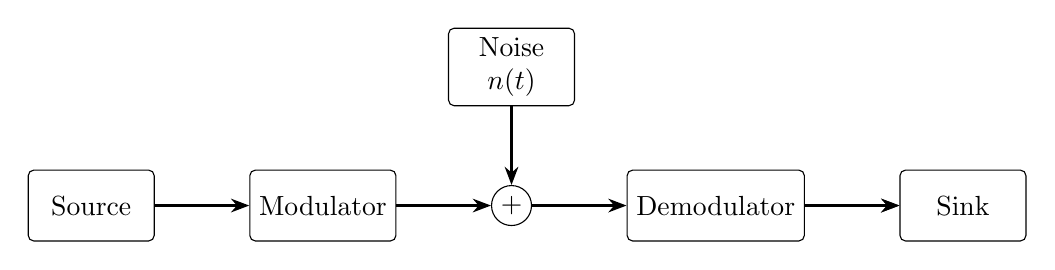
\begin{tikzpicture}[
  >=Stealth,
  block/.style = {draw, rounded corners=2pt, minimum height=9mm, minimum width=16mm, align=center},
  sum/.style   = {draw, circle, inner sep=1.5pt, minimum size=4mm},
  line/.style  = {->, thick},
  note/.style  = {font=\scriptsize, inner sep=1pt},
  node distance=10mm and 12mm
]

% Nodes
\node[block]            (src)   {Source};
\node[block, right = of src] (mod)   {Modulator};
\node[sum, right = of mod] (plus) {$+$};
\node[block, right = of plus] (demod) {Demodulator};
\node[block, right=of demod]   (sink)  {Sink};

% Noise source
\node[block, above=of plus] (noise) {Noise\\$n(t)$};

% Connections (TX path)
\draw[line] (src) -- (mod);


% Channel: signal path via adder
\draw[line] (mod.east) -- ++(6mm,0) |- (plus.west);
\draw[line] (plus) -- (demod.west);

% Noise injection
\draw[line] (noise) -- (plus);

% RX path
\draw[line] (demod.east) -- (sink.west);
\draw[line] (demod) -- (sink);

\end{tikzpicture}
\end{document}
